\documentclass[10pt]{examdesign}
\usepackage{amsmath}
\usepackage{enumitem}
\usepackage{amsfonts}
\usepackage{pgfplots}
\usepackage{pifont}
\usepackage{graphicx}
\usepackage{fancyhdr}
\usepackage{cancel}
\usepackage{gensymb}
\usepackage[american]{circuitikz}

\SectionFont{\large\sffamily}
\Fullpages
\ContinuousNumbering
\usepackage{ulem}
\ProportionalBlanks{2}


\DefineAnswerWrapper{}{}
\NumberOfVersions{1}
%\IncludeFromFile{foobar.tex}
\examname{\Large{Inclined Planes}}
\class {\Large Physics}

\def \namedata {Name: \hrulefill\\ 
	Date: \hrulefill \\
	Period: \hrulefill \\
	Primary Peer Reviewer: \hrulefill 
	\\
			\begin{tabular}{| p{1cm} | p{1cm} | p{1 cm} | p{1cm} |}
	\hline
		+1 & 0 & -1 & $\Sigma$ 
		\\
		\hline
		& & & \vspace{.5cm}
		\\ \hline
	
	\end{tabular}
	\\
 \vspace{-.6in}
	
}




\begin{document}




\begin{multiplechoice} [title={Multiple Choice},
	rearrange=no]


	
	\begin{question}
In general, which coordinate system would be best for working with an inclined plane?
\choice{+x: To the Right; +y: Down}
\choice{+x: To the Left; +y: Up}
\choice{+x: Up the ramp  +y: Perpendicular to the ramp, in the direction of the normal force.}
\choice{+x: Up the ramp  +y: to the right}
\choice{+x: Down the Ramp  +y: To the Left}
	\end{question}

\begin{block}
\textbf{	Questions 2-4 refer to the following information:}
	

		\hspace{2in}	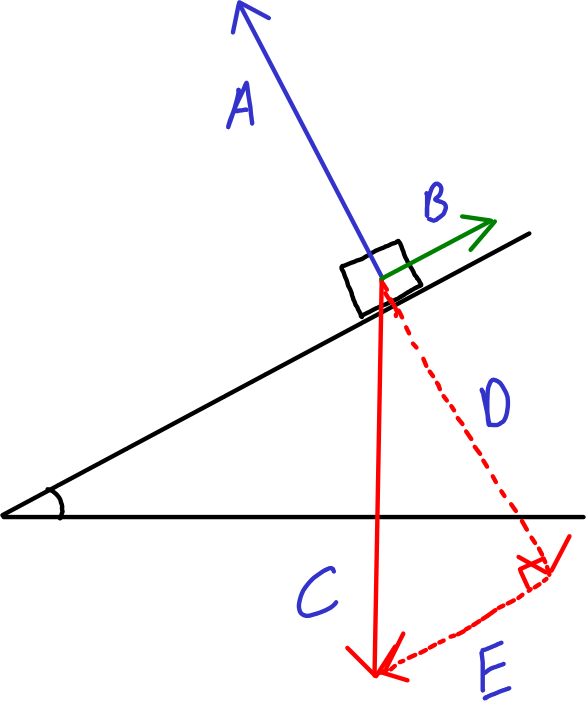
\includegraphics[height=1.75in]{inclinedplane.png}


	
	
	
	\begin{question}
		On the diagram above, which arrow best represents the component of gravity that is parallel to the plane?
		\choice{A}
		\choice{B}
		\choice{C}
		\choice{D}
		\choice{E}
		\end{question}
	
		\begin{question}
		On the diagram above, The arrow labeled \textit{A} represents - 
		\choice{the natural force.}
		\choice{The weight of the object.}
		\choice{The normal force.}
		\choice{Friction}
		\choice{The component of gravity that is perpendicular to the plane.}
	\end{question}


			\begin{question}
		On the diagram above, The arrow labeled \textit{B} represents - 
		\choice{the natural force.}
		\choice{The weight of the object.}
		\choice{The normal force.}
		\choice{Friction}
		\choice{The component of gravity that is parallel to the plane.}
	\end{question}
		
	\end{block}
\end{multiplechoice}

\begin{multiplechoice} [title={Multiple Correct Multiple Choice}]
\textit{	For each question, please choose TWO correct answers.  No credit will be given for incorrect or partially correct answers. }

	\begin{question}
	Which of the following statements are true concerning the normal force? (Choose TWO)
	\choice{The normal force is always directed upward.}
	\choice{The normal force always cancels friction.}
	\choice{The normal force and gravity always completely cancel.}
	\choice{The normal force is always directed perpendicular to a surface.}
	\choice{The normal force and the component of gravity that is perpendicular to the surface are in exactly opposte directions.}
\end{question}


\end{multiplechoice}

\begin{shortanswer}  [title={Free Response}, rearrange=no]
	
\begin{center}
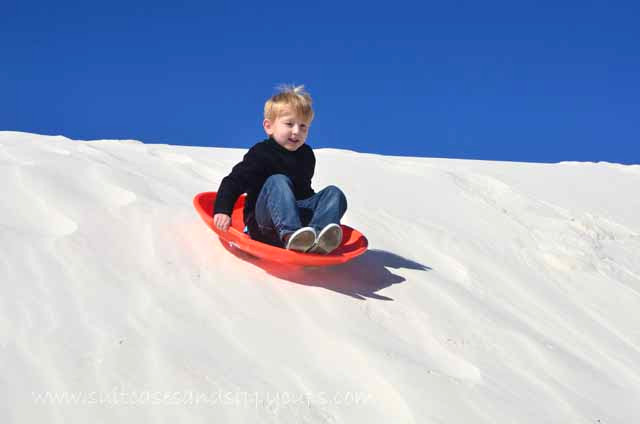
\includegraphics[height=1.5in]{DSC_3566.jpg}
\end{center}


	\begin{question}
	A child is riding down a dune at White Sands National Monument on a sand sled, as shown in the picture above.  The mass of the child is 20 kg, and the angle of the hill is 33\degree.   If the child accelerates at a rate of 2.843 m/s\textsuperscript{2}, what is the force of friction that acts on the child? 
	\end{question}
	
	\end{shortanswer}



\end{document}


